\documentclass[12pt, letterpaper]{article}
\usepackage[utf8]{inputenc}
\usepackage{amsmath}
\usepackage{booktabs}
\usepackage{parskip}

\usepackage{graphicx}
\graphicspath{{../images/}}

\usepackage{hyperref}
\hypersetup{
    colorlinks=true,
    urlcolor=blue,
    linkcolor=blue,
    citecolor=blue,
    filecolor=blue,
}
\urlstyle{same}

\title{Notes to Results}
\author{}
\date{}


\begin{document}
\maketitle

\section{Predictive Performance}



\section{Explanations and Interpretation}

Interpreting the results of high-dimensional and complex statistical models is notoriously difficult.
This section approaches the challenge from two opposite angles.

First, we reduce the \emph{complexity} by fitting a simple and well-understood Linear Regression Model with the same features that were selected for the best-performing Neural Network and analyze the coefficients.

Second, we reduce the \emph{dimensionality} by leveraging a different Neural Network and visualize the results in two-dimensional space.

\subsection{Feature Importance}

In order to draw conclusions about which features were most important for the Neural Network one could imagine to compute gradients of the single output node with respect to each input node by backpropagating through the entire network.
We chose to analyze the feature importance of an auxiliary Linear Regression model instead to provide some suggestions that could potentially apply to the Neural Network as well.

Therefore we preselected $25$ of the network's input features with the \texttt{RFE} algorithm introduced in the previous chapter and compared the coefficient magnitudes.
As noted before, all predictors were standardized such that a meaningful comparison is feasible.

The results are shown in figure \ref{fig:coefficient-plot}.
It is worth noting that the two most important features based on various different feature selectors of the \texttt{scikit-learn} library were always the number of \emph{bedrooms} and the (number of) \emph{accomodates} in this order, both measuring the apartment's \emph{capacity}.

The coefficient plot, however, is dominated by categorical features:
In agreement with human intuition the \emph{room} type, the \emph{property} type and the \emph{neighbourhood} strongly influence the predicted price.
Unsurprisingly, the property types \emph{entire home} and \emph{entire villa} are connected with high prices, whereas the the room type \emph{shared room} correlates with cheaper apartments.
Notably, the price predictions from the Convolutional Network fitted on the image data indicates a significant positive effect, conditioned on all other selected features.

When analyzing the \emph{marginal} effect of neighbourhood on price by e.g. ordering the neighbourhoods according to their median price, this order is nearly identical to the ranking in figure \ref{fig:coefficient-plot} with \emph{Frogner} at the top and \emph{Grorud} at the bottom.

Interestingly, apartments in the \emph{Sentrum} (central area) have a large positive coefficient in the regression, yet the second to lowest median price.
This finding indicates the presence of \emph{confounders}:
The city center might plausibly be connected to fewer rooms and smaller apartment sizes overall pulling the median price down.
These confounding effects are controlled for in the regression model but not in the naive bivariate analysis.


\subsection{Sensitivity to Outliers}

% Manually constructed with saved .csv file in tables folder and
% https://www.tablesgenerator.com/latex_tables
\begin{table}[t]
    \centering
    \begin{tabular}{@{}ccc@{}}
        \toprule
        \textbf{Quantile Threshold} & \textbf{MAE} & \textbf{$R^2$} \\ \midrule
        0.0                         & 443.35       & 0.16           \\
        1.0                         & 337.59       & 0.51           \\
        2.5                         & 282.17       & 0.53           \\
        5.0                         & 240.57       & 0.54           \\
        10.0                        & 214.76       & 0.49           \\ \bottomrule
    \end{tabular}
    \caption{Mean Absolute Error and $R^2$ value of the Neural Network on the validation set after removing the highest quantiles of the price distribution from the data set}
    \label{tab:mlp-outliers}
\end{table}

Table \ref{tab:mlp-outliers} shows performance metrics for the Neural Network fitted on a subset of the data in the validation set.
As indicated by the first column the dataset was reduced by successively cutting off observations from the top of the price distribution.
More precisely, the first row refers to the entire data whereas the last row excludes the top $10$\% most expensive apartments.

By omitting just the top $1$\%, the MAE reduces by over $100$ NOK (about $10$ Euros) and the $R^2$ rapidly jumps to over $0.5$.
This sensitivity to outliers in the price distribution is \textbf{not} solved by log-transforming the price, all classical models from the previous chapter suffer from the same effect.

Clearly, the Neural Network lacks the ability to capture the entire price range accurately.
There are two possible explanations for this phenomenon:
%%%
\begin{enumerate}
    \item The model is flawed.
    \item The model is faced with a nearly impossible task.
\end{enumerate}
%%%
In order to discriminate the observations with the highest prices from all other listings, the corresponding feature combinations must be separable in the $59$-dimensional feature space.
Since this high-dimensional space cannot be visualized, we approximate it with an two-dimensional \emph{embedding} or \emph{latent space}.
If the price outliers are clearly separated from the rest in this embedded space, the network is faced with a feasible task.
If, however, the outliers are located in the \emph{middle} of the latent distribution, there is little hope to discriminate the most expensive apartments from any of their potentially much lower priced embedded neighbours.
In this case, the collected data might simply not be rich or expressive enough to capture all factors that contribute to very high prices.

Modern Machine Learning methods provide a large toolbox for low-dimensional embeddings.
Since the project is mainly focused on Deep Learning we decided to use a \emph{Variatonal Autoencoder}.
In contrast to deterministic Autoencoders the VAE contains an additional loss term apart from the usual reconstruction loss that pulls the encoded latent space distribution towards an isotropic multivariate Gaussian distribution.
For this reason, latent space visualizations of the VAE appear to be more spread out and output classes (that are not used for training the VAE) tend to be easier to identify.

%%%
\begin{figure}[t]
    \centering
    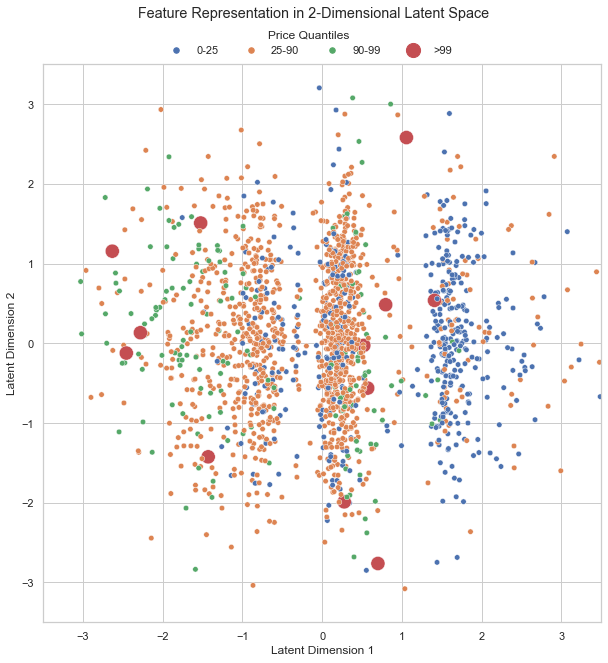
\includegraphics[width=0.8\textwidth]{latent_representation.png}
    \caption{Feature Representation in a two-dimensional latent space embedding}
    \label{fig:latent-representation}
\end{figure}
%%%

Figure \ref{fig:latent-representation} visualizes the two-dimensional feature embedding.
Already a \emph{single} dimension seems so be sufficient for a general understanding of price segments.
While some of the most expensive apartments are located on the far left, surrounded by highly-priced neighbours, the other half shares a similar feature representation to \emph{medium to low} priced listings.
Hence, the network likely maps this second half to comparably low price predictions resulting in large residuals with a high influence on the MAE and the $R^2$ value.

Finally, it can be argued that the entire task of predicting Airbnb prices is flawed in the first place.
In order to draw connections from features to outputs the process implicitly assumes observations whose listed price can be justified and explained by characteristics of the joint feature distribution.

In practice, however, some apartments might be drastically overpriced biasing the model to learn wrong feature-price mappings and inflating the error metrics.
Such observations are extremely hard to detect:
While some covariates might be able to accurately approximate low demand, the corresponding apartment could be undesirable for other reasons than its price.
In fact, even a price outlier with zero guests can be well worth the money, yet nobody is willing to pay that high amount for an accomodation, regardless of its quality.
As a consequence, a blind removal of such outliers is difficult to justify when obeying correct statistical methodology.

\newpage

\bibliography{bib}
\bibliographystyle{apalike}

\appendix

%%%
\begin{figure}[t]
    \centering
    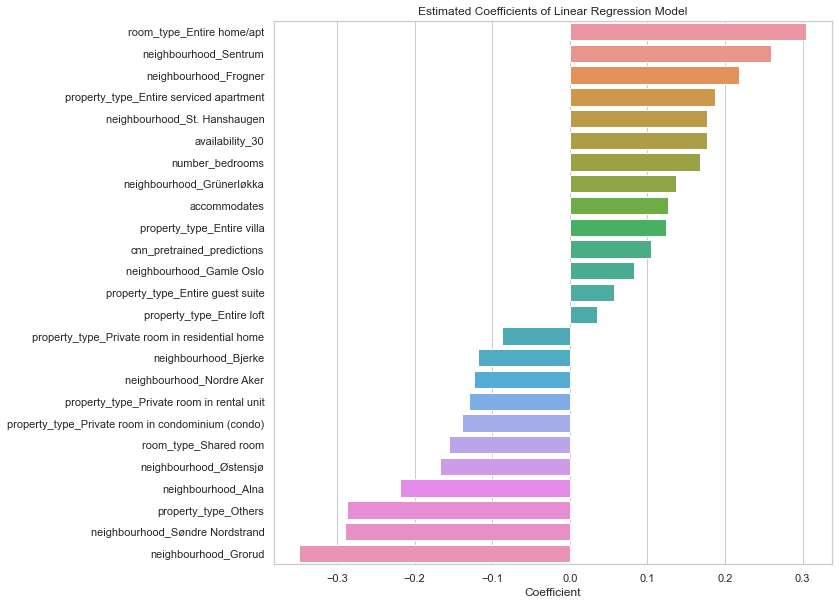
\includegraphics[width=\textwidth]{coefficient_plot.png}
    \caption{Estimated coefficients of a Linear Regression model for $25$ preselected features}
    \label{fig:coefficient-plot}
\end{figure}
%%%

\end{document}